\section{Presentation of the campus}
My internship took place in Japan (\begin{CJK}{UTF8}{min}日本\end{CJK}), in the university of Ritsumeikan on its science-oriented Biwako-Kusatsu campus, in the city of Minami-Kusatsu.
\subsection{Ritsumeikan University}
Ritsumeikan University (\begin{CJK}{UTF8}{min}立命館大学\end{CJK}) is a private school, with about thirty-five thousand students departed in four different campuses.
The main campus, in Kinugasa, was founded in 1869 by Kinmochi Saionji. It is oriented towards litterature, law, history and arts.
\subsubsection{Biwako-Kusatsu Campus}
\begin{figure}[h]
  \centering
  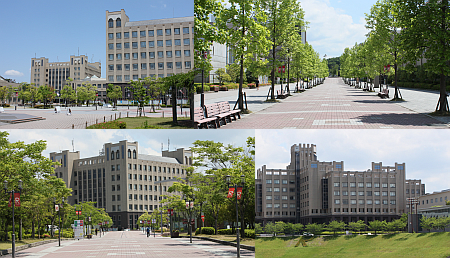
\includegraphics[scale=0.7]{rits1.jpg}
  \caption{Some pictures of the campus}
\end{figure}
The campus is in Minami-Kusatsu, about twenty minutes from train from Kyoto city. My internship took place mostly in the Creation Core building, dedicated to computer science and engineering.
\subsection{The lab system}
From what I understood, every student in engineering and computer science is affected to a laboratory they choose. There are many different labs, and each have a teacher, which teaches a very particular domain to the students in the lab. These students then conduct experiments and write scientific papers. This allows them to become very proficient in a very specific domain, since they spend a lot of time in the lab apart from the courses. Every lab has weekly meetings where every student presents his work for the past week.
\subsection{The Acoustics \& Signal Processing Lab}
\acused{ASPL}
I was a student of the \ac{ASPL} for these three months. The focus of the lab is somewhere between acoustics and \ac{dspg} : some students will do more acoustics, fluid mechanics, etc...  while some others will do more computer science-related work.

The lab website (\url{http://www.aspl.is.ritsumei.ac.jp/}, in Japanese) has information about past and future events, seminars, and papers. 
\subsubsection{Activities}
The research activities include :
\begin{itemize}
\item Parametric loudspeakers
\item Speech recognition
\item Speech resynthesis
\item Reverberation reduction
\item Speech distortion reduction
\item And many more. Each student is affected to a very specific subject.
\end{itemize}

Here are some examples of papers produced this year: \url{http://www.aspl.is.ritsumei.ac.jp/2013paper.htm}.

\subsubsection{Organisation}
The teacher (sensei, \begin{CJK}{UTF8}{min}先生\end{CJK}) and head of the laboratory is Mr. Takanobu Nishiura. There is a secretary, which takes care of the administrative matters, and many common matters of the lab, for instance server maintenance, are resolved by the students.
There are about thirty-five students, whose level range from undergraduate to Ph. D.